\documentclass{beamer}
\usetheme{ODK}
\usepackage{tikz}

\usepackage[utf8]{inputenc}
\usepackage{eurosym}
\usepackage{graphicx}
\graphicspath{{../../../Proposal/Pictures/}}

\makeatletter
\newskip\@bigflushglue \@bigflushglue = -100pt plus 1fil
\def\bigcenter{\trivlist \bigcentering\item\relax}
\def\bigcentering{\let\\\@centercr\rightskip\@bigflushglue%
\leftskip\@bigflushglue
\parindent\z@\parfillskip\z@skip}
\def\endbigcenter{\endtrivlist}
\makeatother

\author{Nicolas M. Thiéry}
\title{OpenDreamKit: an introduction}

\begin{document}

\begin{frame}
  \titlepage

\end{frame}

\begin{frame}{Some fundamental trends}\label{some-fundamental-trends}
\end{frame}

\begin{frame}{Long standing and booming role of computers in pure
    mathematics}
  \label{long-standing-and-booming-role-of-computers-in-pure-mathematics}

  % TODO: not new: Euler / ...

  \begin{itemize}
  \item \textbf{Computer exploration} to discover and check conjectures
  \item \textbf{Assisted, certified, mechanized proofs}: \href{https://coq.inria.fr/}{CoQ}, \href{https://isabelle.in.tum.de/}{Isabelle}, ...
  \item \textbf{Collaborative work}:
    \href{https://www.wikipedia.org/}{Wikipedia},
    \href{https://polymathprojects.org/}{Polymath}, ...
  \item \textbf{Mathematical Knowledge Management}: arXiv, ...
  \item \textbf{Education}
  \end{itemize}
\end{frame}

\begin{frame}{Open Science getting momentum}
  \begin{quote}
    ``\href{https://en.wikipedia.org/wiki/Open_science}{Open science}
    is the movement to make scientific research, data and
    dissemination accessible to all levels of an inquiring society,
    amateur or professional''
  \end{quote}

  \begin{itemize}
  \item Open Knowledge (Access, Educational Ressources)
  \item Open Source or, better, Free Software
  \item Open Data
  \item Open Peer Review, Methodology, ...
  \end{itemize}

  \begin{itemize}
  \item At the core of science for centuries
  \item Finally getting recognition as \textbf{viable} and \textbf{necessary},\\
    even by funding agencies!
  \end{itemize}
\end{frame}

\begin{frame}{Emergence of a vibrant ecosystem of free software for
    pure mathematics}
  \label{emergence-of-a-vibrant-ecosystem-of-free-software-for-pure-mathematics}

  \begin{itemize}
  \item \textbf{Specialized systems}: \href{http://www.linalg.org/}{LinBox},
    \href{http://pari.math.u-bordeaux.fr/}{PARI/GP},
    \href{http://mpir.org/}{MPIR},
    \href{http://www.singular.uni-kl.de/}{Singular}, \ldots{}
  \item \textbf{General purpose systems}: \href{http://www.gap-system.org/}{GAP},
    \href{http://www.sagemath.org/}{SageMath}, \ldots{}
  \item \textbf{Online databases}: \href{https://oeis.org/}{OEIS},
    \href{http://www.lmfdb.org/}{LMFDB}, \ldots{}
  \item \textbf{Interactive computing environments}:\\
    \href{https://jupyter.org/}{Jupyter},
    \href{https://cloud.sagemath.com/}{SageMathCloud}, \ldots{}
  \item Together with the wider \textbf{Scientific Python ecosystem}
  \end{itemize}
  \bigskip\pause

  \begin{block}{Viable alternatives to Maple, Mathematica, Matlab,\ldots{}}
    \label{viable-alternatives-to-maple-mathematica-matlab}
    For research and education (and the industry?)
  \end{block}
\end{frame}


\begin{frame}{Virtual Research Environments (VRE): the next frontier?}

  \begin{block}{H2020 European Research Infrastructures Work Programme}

    \begin{quote}
      ``Groups of researchers, typically widely dispersed who are working
      together through ubiquitous, trusted and easy access to services
      for scientific data, computing, and networking, in a
      \textbf{collaborative virtual environment}``
    \end{quote}
  \end{block}
  \bigskip

  \begin{block}{A useful VRE for mathematics?}
  \end{block}
\end{frame}

\begin{frame}{Mathematicians are already immersed in many VREs}
  \begin{bigcenter}
    \includegraphics[width=\textwidth]{TheBigPictureBefore.pdf}
  \end{bigcenter}
\end{frame}

\begin{frame}{A workflow based VRE?}
  \centerline{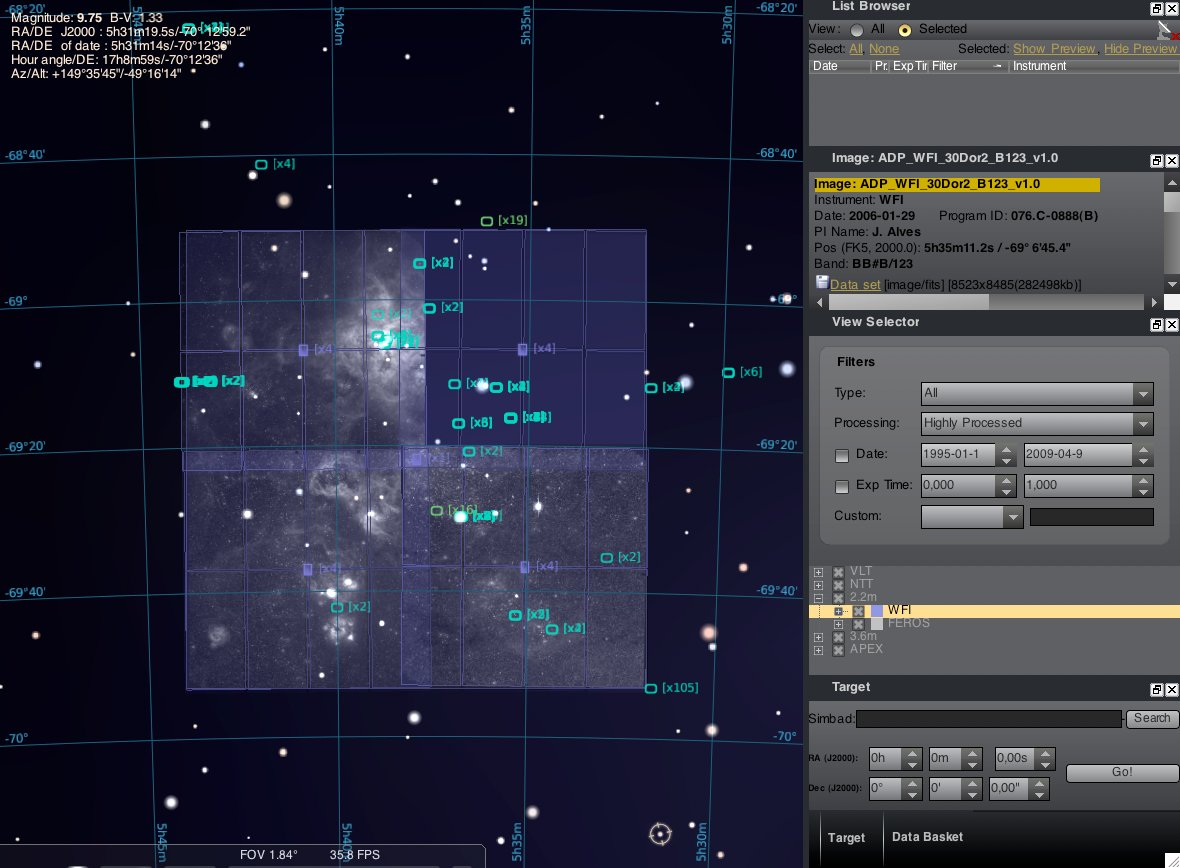
\includegraphics[height=.7\textheight]{virtual_observatory.jpeg}}
  \pause\bigskip

  \centerline{\color{red} Could cover only a tiny fragment of mathematics}
\end{frame}

\begin{frame}{The Read-Eval-Print loop and notebook metaphors}
  \centerline{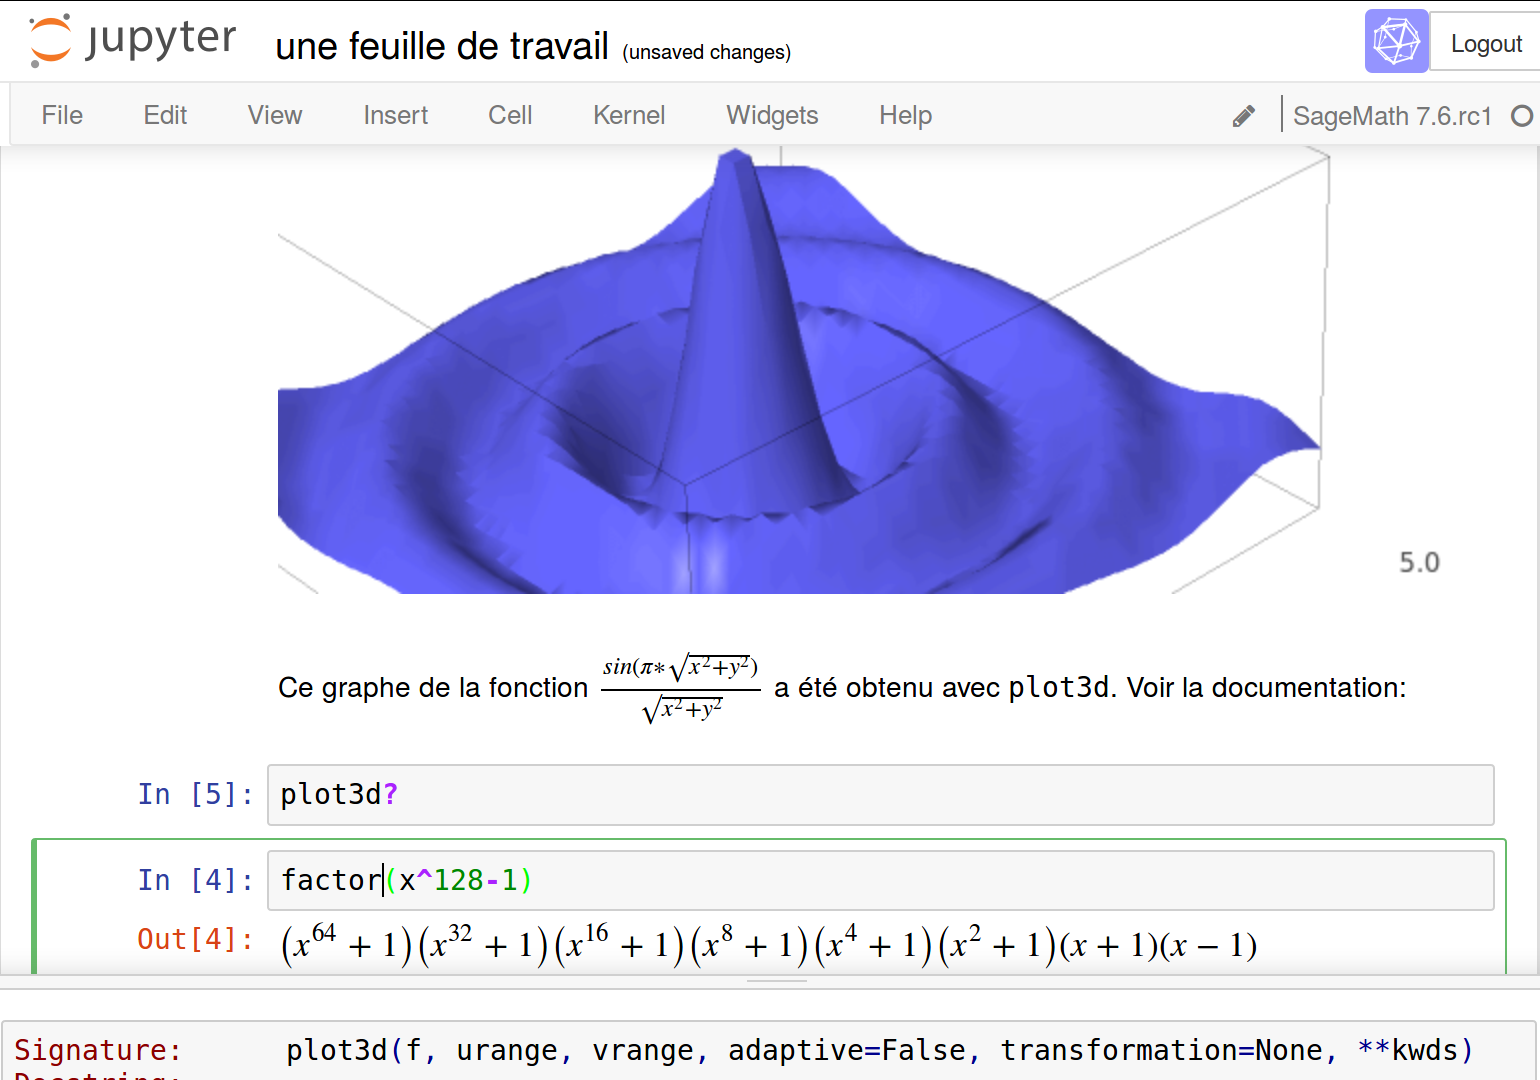
\includegraphics[height=.8\textheight]{worksheet.png}}
\end{frame}

\begin{frame}{A proof of concept VRE: SageMathCloud}
  \centerline{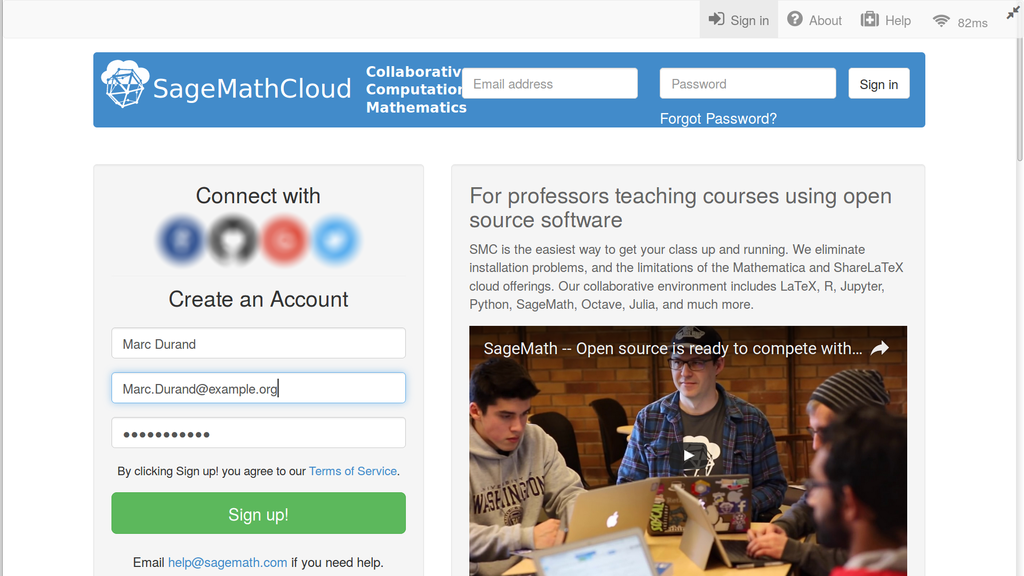
\includegraphics[width=\textwidth]{smc.png}}
\end{frame}

\begin{frame}{A one-size-fits-all VRE?}
  \pause
  \begin{block}{Supporting many scales}
    \begin{itemize}
    \item A single person installation on a laptop
    \item A collaborative VRE between three researchers, running on
      their lab's server
    \item A university wide VRE for teaching
    \item A service provided by a European grid infrastructure
    \end{itemize}
  \end{block}
  \pause

  \begin{block}{Supporting many computational components}
  \end{block}
  \pause

  \begin{block}{Supporting many data bases}
  \end{block}
  \pause

  \centerline{\color{red}Way too many use cases!}
\end{frame}

\begin{frame}{OpenDreamKit's proposal}\label{our-proposal}
  Building a \textbf{VRE Toolkit for Mathematics}
  \pause\bigskip

  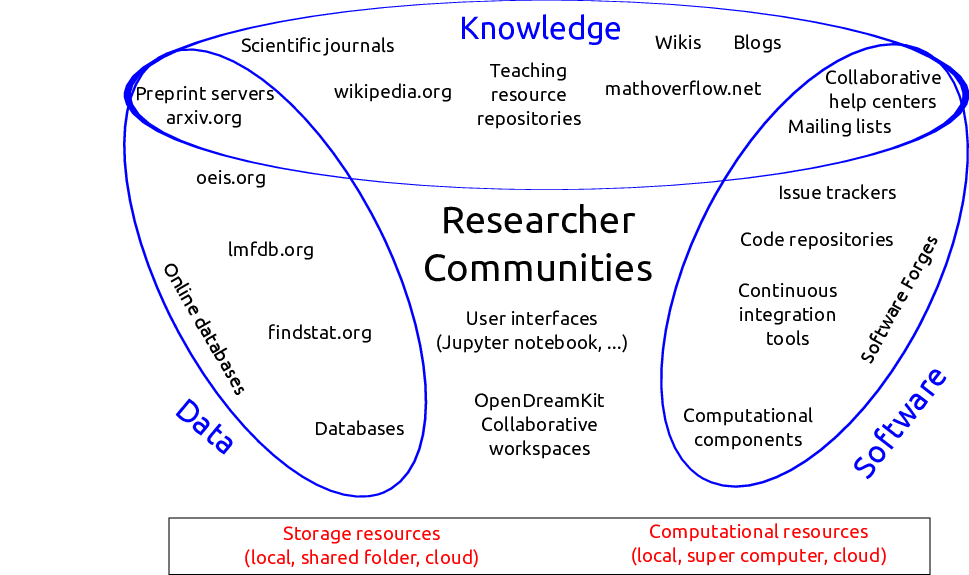
\includegraphics[width=.9\textwidth]{TheBigPicture.pdf}
\end{frame}

\begin{frame}{Added values of the toolkit approach}
  \begin{itemize}
  \item \textbf{Modularity}, \textbf{sustainability}
  \item Joining forces with the wider scientific computing community
  \item Lowering the software barrier between pure and applied maths
  \end{itemize}
\end{frame}


\begin{frame}{Open Digital Research Environment Toolkit for the
    Advancement of Mathematics}

  \begin{itemize}
  \item \href{OpenDreamKit.org}{OpenDreamKit.org}
  \item \href{https://ec.europa.eu/programmes/horizon2020/}{H2020}
    \href{https://ec.europa.eu/programmes/horizon2020/en/h2020-section/european-research-infrastructures-including-e-infrastructures}{European
      Research Infrastructures} Work Programme

    Call: Virtual Research Environments

  \item Budget: 7.6M\euro

  \item \href{http://opendreamkit.org/partners}{18 sites, 50 participants}
  \item In close collaboration with the international community!
  \end{itemize}
\end{frame}

\begin{frame}{A user-driven consortium}

  %\begin{block}
  {European power users and core developers of the
      ecosystem of open source software for Mathematics:}
    \begin{itemize}
    \item GAP (St Andrews, Oxford)
    \item Linbox (Grenoble)
    \item PARI/GP (Bordeaux, Versailles)
    \item SageMath (Bordeaux, Grenoble, Paris Sud, Oxford, Versailles)
    \item Singular (Kaiserslautern)
    \item LMFDB (Warwick, Zürich)
    \item MathHub, MMT/OpenMath (Bremen)
    \item Jupyter (Simula)
    \item Scientific Python (SouthHampton, Sheffield, Silesia)
    \end{itemize}
  %\end{block}
  \pause\medskip
  \begin{block}{Supported by:}
    \begin{itemize}
    \item Research Software Engineers
    \item An open source based company (Logilab)
    \end{itemize}
  \end{block}
\end{frame}

\begin{frame}{OpenDreamKit's aims}
  \begin{itemize}
  \item Improve the productivity of researchers in pure mathematics and
    applications by further promoting collaborations on \textbf{Data},
    \textbf{Knowledge}, and \textbf{Software}
  \item Make it easy for teams of researchers of any size to set up
    custom, collaborative \textbf{Virtual Research Environments}
    tailored to their specific needs, resources and workflows
  \item Support the entire life-cycle of computational work in
    mathematical research, from \textbf{initial exploration} to
    \textbf{publication}, \textbf{teaching}, and \textbf{outreach}
  \end{itemize}
\end{frame}

\begin{frame}{How to get there?}
  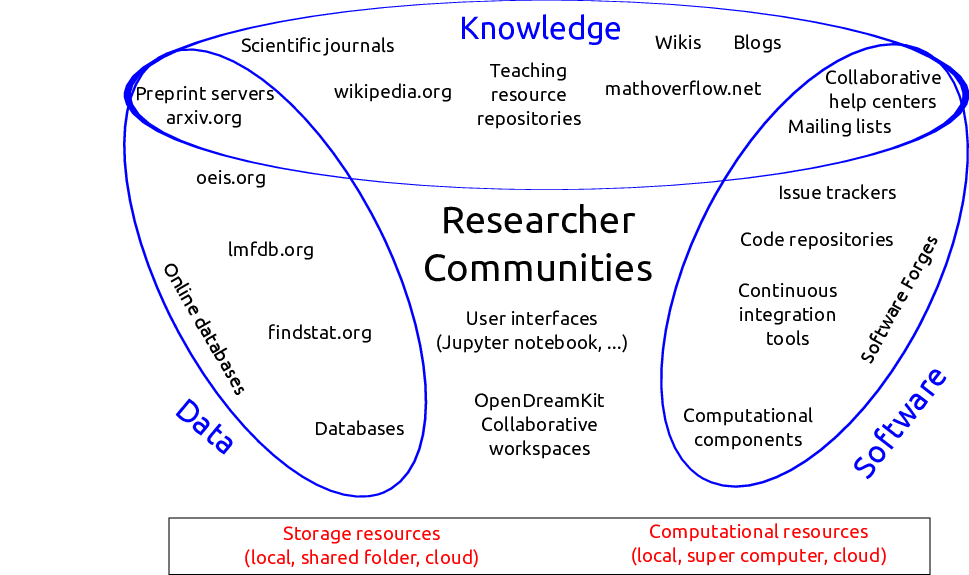
\includegraphics[width=\textwidth]{TheBigPicture.pdf}
\end{frame}

\end{document}

\begin{frame}{Component architecture (WP3)}
  \begin{itemize}
  \item Goal: ease of deployment.
  \item Requires:
    \begin{itemize}
    \item Modularity, packaging, portability, distribution
    \item For individual components and combinations thereof
    \end{itemize}
  \item Development workflows in ecosystems of software
  \end{itemize}
\end{frame}

\begin{frame}{User interfaces (WP4)}
  \label{user-interfaces-wp4}
  \begin{itemize}
  \item Jupyter as uniform notebook interface
  \item Jupyter improvements: interaction, 3D, collaboration, \ldots{}
  \item Collaborative, reproducible, active documents
  \item VRE deployment: JupyterHub, SageMathCloud
  \end{itemize}

  See WP4 presentation
\end{frame}

\begin{frame}{High Performance Mathematical Computing (WP5)}
  \begin{block}{Make the most of available hardware}
    \begin{itemize}
    \item Incore parallelism (SIMD)
    \item Multicore
    \item HPC
    \item cloud
    \end{itemize}
  \end{block}


  \begin{block}{For individual computational components and combinations thereof}
  \end{block}
  See WP5 presentation
\end{frame}

\begin{frame}{Data/Knowledge/Software (WP6)}
  \label{dataknowledgesoftware-wp6}
  \begin{block}{Enable rich and robust interaction between}
    \begin{itemize}
    \item computational components
    \item data bases
    \item knowledge bases
    \item users
    \end{itemize}
  \end{block}
  \begin{block}{Requires}
    \begin{itemize}
    \item explicit common semantic spaces
    \item a language to express them
    \item tools to leverage them
    \end{itemize}
  \end{block}
  \begin{block}{Paradigm shift}
    Drilling much deeper integration into the architecture than
    originally expected
  \end{block}
\end{frame}

\begin{frame}{Community building and dissemination (WP2)}
  \begin{itemize}
  \item Developer workshops
  \item Training workshops and material
  \item Conferences
  \item Communication: blog, web, social media
  \end{itemize}

  See WP2 presentation
\end{frame}

\begin{frame}{Social aspects (WP7)}
  \label{social-aspects-wp7}

  \begin{itemize}
  \item Analysis of user needs
  \item Research on collaborative software development in mathematics
  \end{itemize}
  See WP7 presentation
\end{frame}

\end{document}
